\documentclass[a4paper,10pt]{article}
\usepackage[utf8]{inputenc}
\usepackage[francais]{babel}
\usepackage{indentfirst}
\usepackage{listings}
\usepackage{graphicx}
\usepackage{blindtext}
\usepackage{enumitem}
\usepackage{hyperref}
\usepackage{algorithm}
\usepackage{amsmath}
\usepackage[top=2.5cm,bottom=2.5cm,left=2.5cm,right=2.5cm]{geometry}
\pagestyle{headings}
\title{Projet : INFO-F-302 Informatique Fondamentale.}
\author{George Rusu et Maximilien Romain}
\date{\today}
\begin{document}
\maketitle
\tableofcontents
\newpage
\section{Introduction}
Le premier objectif de ce projet est de modeliser divers problemes en problemes de satisfaction de contraintes (CSP). Le second objectif est d’implementer un programme resolvant ces problemes en utilisant ChocoSolver.

\textbf{link} :  http://www-master.ufr-info-p6.jussieu.fr/2005/IMG/pdf/rp3.pdf

\section{Question 1}
L'ensemble des cases du jeux $V$ où $ \#V = n^2$ \\
\textbf {Variables de décision} $ X = \{x_{i,j} | \forall i,j (1 \leq i \leq n).(1 \leq j \leq n)\}$ , $n^2$ variables de décision \\
\textbf{Domaines : } $ D = \{vide, fous, cavalier, tour\} $\\
\textbf{Contraintes : } Pour chacune des pièces de l'echequier, si une case est occupé par un pions, alors dans la porté de ce pion, donc les cases attaquables par ce pion, doivent être obligatoirement vide.  On parcours donc chaque case, et lorsque qu'une case est occupé, en fonction du pion qui occupe cette case, les contraintes changent.


\subsection{Contraintes tour}
	Pour chaque colonne de l'echequier, si une case de cette colonne est occupée par une tour, alors le reste des cases de cette colonne doivent être vide:
$$ c_{T_{col},j} = ((x_{1,j}, x_{2,j},\ldots, x_{n,j}), \{(b_1, b_2,\ldots, b_n) | b_i = T, b_j = V, \forall j \ne i\})$$
	Pour chaque ligne de l'echequier, si une case de cette ligne est occupée par une tour, alors le reste des cases de cette ligne doivent être vide:
$$ c_{T_{i,ligne}} = ((x_{i,1}, x_{i,2},\ldots, x_{i,n}), \{(b_1, b_2,\ldots, b_n) | b_i = T, b_j = V, \forall j \ne i\})$$

\subsection{Contraintes fou}
	Les contraintes du fou sont composées dans le même état d'esprit que les contraintes des tours, cepandant la portée d'un fou change, et en fonction de la digonale sur laquelle est placé le fou, la distance maximal que ce fou peut atteindre change.  En effet les plus grand diagonales se trouve en $(0,0)$ et $(0,n-1)$.
	Par contrainte, on considère toujours la diagonale opposée, et on réunie les deux diagonales par un \emph{and}.

$$ c_{F,2*n-2} = ((x_{1,n-1}, x_{2,n}), \{(b_1, b_2)| b_1 = F, b_2 = V \lor b_1 = V, b_2 = F\})\land$$ $$((x_{1,2}, x_{2,1}), \{(b_1, b_2)| b_1 = F, b_2 = V \lor b_1 = V, b_2 = F\}) $$ 
{\centering
  \vdots\par
}
$$ c_{F,n+1} = ((x_{1,2}, x_{2,3}, \ldots, x_{n-1,n}), \{(b_1, b_2, \ldots, b_{n-1})|b_i = F, b_j = V, \forall j \ne i\}) \land$$ $$((x_{1,n-1},x_{2,n-2}, \ldots, x_{n-1,1}), \{(b_1, b_2, \ldots, b_{n-1})|b_i = F, b_j = V, \forall j \ne i\}) $$
$$ c_{F,n} = ((x_{1,1}, x_{2,2},\ldots, x_{n,n}), \{(b_1, b_2, \ldots, b_n)|b_i = F, b_j = V, \forall j \ne i\}) \land$$ $$((x_{1,n}, x_{2,n-1}, \ldots, x_{n, 1}), \{(b_1, b_2, \ldots, b_n)|b_i = F, b_j = V, \forall j \ne i\})$$
$$ c_{F,n-1} = ((x_{2,1}, x_{3,2},\ldots, x_{n, n-1}), \{(b_1, b_2, \ldots, b_{n-1})|b_i = F, b_j = V, \forall j \ne i\}) \land$$ $$((x_{2,n}, x_{3,n-1}, \ldots, x_{n,2}), \{(b_1, b_2, \ldots, b_{n-1})|b_i = F, b_j = V, \forall j \ne i\}) $$
{\centering
  \vdots\par
}
$$ c_{F,2} = ((x_{n-1,1}, x_{n,2}), \{(b_1, b_2)| b_1 = F, b_2 = V \lor b_1 = V, b_2 = F\}) \land$$ $$((x_{n-1,n}, x_{n,n-1}), \{(b_1, b_2)|b_1 = F, b_2 = V \lor b_1 = V, b_2 = F\}) $$

	Les diagonales de gauche à droite sont représenté par la matrice ci-dessous.
\begin{equation}
\left( \begin{array}{ccccc}
c_{F,n} & c_{F,n+1} & \dots & c_{F,2*n-2} & \hfill \\
c_{F,n-1} & c_{F,n} & c_{F,n+1} & \vdots&  c_{F,2*n-2}\\
\vdots & c_{F,n-1} & c_{F,n} &c_{F,n+1} & \vdots \\
c_{F,2}& \vdots & c_{F,n-1}& c_{F,n} &c_{F,n+1} \\
\hfill & c_{F,2} & \dots& c_{F,n-1} & c_{F,n} \\
\end{array} \right)
\end{equation}

\subsection{Contraintes cavalier:}
	Les contraintes des cavaliers sont plus simple. En effet si on rencontre une case occupée par un cavalier, alors il n'y a que 8 contraintes pour les 8 cases que le cavalier peut atteindre.  Si le cavalier est en $(i,j)$, alors il ne peut qu'attaquer les cases où $i+e,j+e, e \in [+1,-1,+2,-2]$
$$ c_{C,(i,j)} = ((x_{i,j}, x_{i+1,j+2}, x_{i+1,j-2}, x_{i-1,j+2}, x_{i-1,j-2}, x_{i+2,j+1}, x_{i+2,j-1}, x_{i-2,j+1}, x_{i-2,j-1}),$$ $$\{(b_1, b_2, \ldots, b_9)|b_1 = C, b_2, \ldots b_9 = V\}) $$


\section{Question 2}
L'ensemble des cases du jeux $V$ où $ \#V = n^2$ \\
\textbf {Variables de décision} $ X = \{x_{i,j} | \forall i,j (1 \leq i \leq n).(1 \leq j \leq n)\}$ , $n^2$ variables de décision \\
\textbf{Domaines : }
$ D = \{Vide, tour, fous, cavalier \} $\\
\textbf{Contraintes : } Pour chacune des pièces de l'echequier, si une case est vide, alors il existe au moins un pion qui menace cette case vide

\subsection{Contraintes tours}
	Pour chaque case de l'echequier qui n'est pas occupé par un pion, alors il existe au moins une tour dans la ligne ou la colonne de la case non occupée.
$$ c_T = ((x_{i,j}, \forall i,j (1 \leq i \leq n).(1 \leq j \leq n)),$$ $$\{b_{i,j}, \forall i,j (1 \leq i \leq n).(1 \leq j \leq n)|b_{i,j} = V, \forall l, (1 \leq l \leq n) \exists b_{l,j} = T \lor b_{i,j} = V, \forall k (1 \leq k \leq n), \exists b_{i,k} = T\})  $$
	Nous devons aussi indiqué qu'il n'y pas d'autre pion entre la case vide et la tour.  On indique donc que les cases entre la case vide et la case occupé par une tour, doivent non occupées. Nous avons donc une telle contrainte pour la ligne et la colonne de la case vide menacé par une tour.
%$$ c_{couple,T} = ((x_{i,j}, x_{l,k}), \{(b_{i,j}, b_{l,k})|b_{i,j} = T, b_{l,k} = V, \rightarrow b_{i,m} \forall m (j < m < k), b_{i,m} = V \} \lor$$ $$b_{i,j} = T, b_{l,k} = V, \rightarrow b_{m,j} \forall m (i < m < l), b_{m,j} = V) $$
$$ c_{couple,T_{colonnes}} = ((x_{i,j}, x_{l,j}), \{(b_{i,j}, b_{l,j})|b_{i,j} = T, b_{l,j} = V, \rightarrow b_{m,j} \forall m (i < m < l), b_{m,j} = V \})$$
$$ c_{couple,T_{lignes}} = ((x_{i,j}, x_{i,k}), \{(b_{i,j}, b_{i,k})|b_{i,j} = T, b_{i,k} = V, \rightarrow b_{i,m} \forall m (j < m < k), b_{i,m} = V \})$$

\subsection{Contraintes fous}
	Pour chaque case de l'echequier qui n'est pas occupé par un pion, alors il existe au moins un fou dans les deux diagonales de la case vide.
$$ c_F = ((x_{i,j}, \forall i,j (1 \leq i \leq n).(1 \leq j \leq n)),$$ $$\{b_{i,j},\forall i,j (1 \leq i \leq n).(1 \leq j \leq n)|b_{i,j} = V, \forall l,k (1 \leq l \leq n).(1 \leq k \leq n) \exists b_{l,k} = F \lor$$ $$b_{i,j} = V, \forall l,k (1 \leq l \leq n).(n \leq k \leq 1), \exists b_{l,k} = F\})  $$
	De nouveau nous devons nous assurer qu'il n'y a pas d'autre pions qui gène le fou entre la case vide et ce fou.
$$ c_{couple,F_{diag1}} = ((x_{i,j}, x_{l,k}), \{(b_{i,j}, b_{l,k})|b_{i,j} = T, b_{l,k} = V, \rightarrow b_{x,y} \forall x,y (i < x < l).(j < y < k), b_{x,y} = V \})$$
$$ c_{couple,F_{diag2}} = ((x_{i,j}, x_{l,k}), \{(b_{i,j}, b_{l,k})|b_{i,j} = T, b_{l,k} = V, \rightarrow b_{x,y} \forall x,y (i < x < l).(k < y < j), b_{x,y} = V \})$$

\subsection{Contraintes cavaliers:}
		Pour chaque case de l'echequier qui n'est pas occupé par un pion, alors il existe au moins un cavalier qui menace la case vide. Pour cela il suffit de verifier qu'il existe une case dans les 8 cases correspondant à l'ensemble des mouvements du cavalier ($\{+1,-1,+2,-2\}$), soit occupé par un cavalier.
$$ c_{C,(i,j)} = ((x_{i,j}, x_{i+1,j+2}, x_{i+1,j-2}, x_{i-1,j+2}, x_{i-1,j-2}, x_{i+2,j+1}, x_{i+2,j-1}, x_{i-2,j+1}, x_{i-2,j-1}),$$ $$\{(b_1, b_2, \ldots, b_9)|b_1 = V, \forall i,j \in [+1,+2,-1,-2], \exists b_{i,j} = C\}) $$

\subsection{Contrainte finale:}
	Finalement il n'y a qu'une seule grande contrainte à appliquer à notre problème. Etant donné qu'il suffit qu'un seule pion menace une case vide, nous pouvons relier nos contrainte par des conditions \emph{or}. 
$$ C = (C_T \land c_{couple,T_{colonnes}} \land c_{couple,T_{lignes}}) \lor (c_F \land c_{couple,F_{diag1}} \land c_{couple,F_{diag2}}) \lor c_{C,(i,j)}$$

\section{Question 2 avec ensemble}
L'ensemble des cases du jeux $V$ où $ \#V = n^2$ \\
\textbf {Variables de décision} $ X = \{x_{i,j} | \forall i,j (1 \leq i \leq n).(1 \leq j \leq n)\}$ , $n^2$ variables de décision \\
\textbf{Domaines : }
$ D = \{Vide, tour, fous, cavalier \} $\\
\textbf{Contraintes : } Pour chacune des pièces de l'echequier, si une case est vide, alors il existe au moins un pion qui menace cette case vide.  Le problème ici, est que nous devons trouver un moyen d'appliquer un \emph{OR} de contraintes, ce qui n'est pas possible.  Nous allons donc définir divers ensemble, et ensuite écrire une grande contrainte appliquant des \emph{Unions} de ces ensembles.

	\subsection{Ensemble Tours}
		Pour chaque case de l'echequier qui n'est pas occupé par un pion, alors il existe au moins une tour dans la ligne ou la colonne de la case non occupée.
		$$ e_T = \{(x_{i,j}, \forall i,j (1 \leq i \leq n).(1 \leq j \leq n)),$$ $$\{b_{i,j}, \forall i,j (1 \leq i \leq n).(1 \leq j \leq n)|b_{i,j} = V, \forall l, (1 \leq l \leq n) \exists b_{l,j} = T \lor b_{i,j} = V, \forall k (1 \leq k \leq n), \exists b_{i,k} = T\}\}  $$
			Nous devons aussi indiqué qu'il n'y pas d'autre pion entre la case vide et la tour.  On indique donc que les cases entre la case vide et la case occupé par une tour, doivent non occupées. Nous avons donc une telle contrainte pour la ligne et la colonne de la case vide menacé par une tour.
		%$$ c_{couple,T} = ((x_{i,j}, x_{l,k}), \{(b_{i,j}, b_{l,k})|b_{i,j} = T, b_{l,k} = V, \rightarrow b_{i,m} \forall m (j < m < k), b_{i,m} = V \} \lor$$ $$b_{i,j} = T, b_{l,k} = V, \rightarrow b_{m,j} \forall m (i < m < l), b_{m,j} = V) $$
		$$ e_{couple,T_{colonnes}} = \{(x_{i,j}, x_{l,j}), \{(b_{i,j}, b_{l,j})|(b_{i,j} = T, b_{l,j} = V) \land ( \forall m (i < m < l), b_{m,j} = V) \}\}$$
		$$ e_{couple,T_{lignes}} = \{(x_{i,j}, x_{i,k}), \{(b_{i,j}, b_{i,k})|(b_{i,j} = T, b_{i,k} = V) \land ( \forall m (j < m < k), b_{i,m} = V) \}\}$$

	\subsection{Ensemble fous}
		Pour chaque case de l'echequier qui n'est pas occupé par un pion, alors il existe au moins un fou dans les deux diagonales de la case vide.
		$$ e_F = \{(x_{i,j}, \forall i,j (1 \leq i \leq n).(1 \leq j \leq n)),$$ $$\{b_{i,j},\forall i,j (1 \leq i \leq n).(1 \leq j \leq n)|b_{i,j} = V, \forall l,k (1 \leq l \leq n).(1 \leq k \leq n) \exists b_{l,k} = F \lor$$ $$b_{i,j} = V, \forall l,k (1 \leq l \leq n).(n \leq k \leq 1), \exists b_{l,k} = F\}\}  $$
			De nouveau nous devons nous assurer qu'il n'y a pas d'autre pions qui gène le fou entre la case vide et ce fou.
		$$ e_{couple,F_{diag1}} = \{(x_{i,j}, x_{l,k}), \{(b_{i,j}, b_{l,k})|(b_{i,j} = T, b_{l,k} = V) \land ( \forall x,y (i < x < l).(j < y < k), b_{x,y} = V) \}\}$$
		$$ e_{couple,F_{diag2}} = \{(x_{i,j}, x_{l,k}), \{(b_{i,j}, b_{l,k})|(b_{i,j} = T, b_{l,k} = V) \land ( \forall x,y (i < x < l).(k < y < j), b_{x,y} = V) \}\}$$

	\subsection{Ensemble cavaliers:}
			Pour chaque case de l'échiquier qui n'est pas occupé par un pion, alors il existe au moins un cavalier qui menace la case vide. Pour cela il suffit de verifier qu'il existe une case dans les 8 cases correspondant à l'ensemble des mouvements du cavalier ($\{+1,-1,+2,-2\}$), soit occupé par un cavalier.
	$$ e_{C,(i,j)} = \{(x_{i,j}, x_{i+1,j+2}, x_{i+1,j-2}, x_{i-1,j+2}, x_{i-1,j-2}, x_{i+2,j+1}, x_{i+2,j-1}, x_{i-2,j+1}, x_{i-2,j-1}),$$ $$\{(b_1, b_2, \ldots, b_9)|b_1 = V, \forall i,j \in \{+1,+2,-1,-2\}, \exists b_{i,j} = C\}\} $$

	\subsection{Contrainte finale:}
		Finalement il n'y a qu'une seule grande contrainte à appliquer à notre problème. Etant donné qu'il suffit qu'un seule pion menace une case vide, nous pouvons relier nos ensemble par des \emph{unions} $\cup$ et des \emph{intersections} de contraintes $\cap$. 
	$$ C = (e_T \cap e_{couple,T_{colonnes}} \cap e_{couple,T_{lignes}}) \cup (e_F \cap e_{couple,F_{diag1}} \cap e_{couple,F_{diag2}}) \cup e_{C,(i,j)}$$

\section{Question 3}
\par Pour cette question nous avons du implementer les deux problèmes décrit ci-dessus. Nous sommes tout d'abord parti sur le fait d'utiliser une matrice de IntVar où chaque case prendrait un numero distinct. Nous nous sommes vites rendu compte que cela n'était pas du tout lisible est très difficile à debugger. Après de nombreuse recherches et de nombreuse questions posées à l'assistant, nous avons eu le déclic que le problème de domination est l'inverse de l'indépendance. En effet, si une pièce menace une autre, il s'agit du problème de domination et inversement pour le problème d'indépendance, une pièce ne doit pas menacer une autre. La negation fait donc son apparition.
\par Pour pouvoir utiliser ce concept avec la negation, nous avions du changer notre premier mode de representation à savoir celui avec un échiquier de taille $n*n$ où chaque case peut-être soit une Tour, soit un Cavalier, soit un Fou, soit un Vide. Nous nous sommes orienté vers la programmation Orienté Objet. Nous avons decider que puisque on va manipuler des pièces, on pourrait créer une classe Piece qui représenterai une pièce du Jeu. Mais chaque type de pièce a son propre espace de jeu ( ses propres contraintes sur les mouvements), nous avons donc du faire de cette classe Piece une classe abstraite afin de pouvoir pour chaque type redéfinir son espace de jeu.
	
\subsection{Lancement du programme}
\par Lors du lancement du jeu, il faut choisir les paramètres en ligne de commande de la manière suivante :
\begin{figure}[!h]
  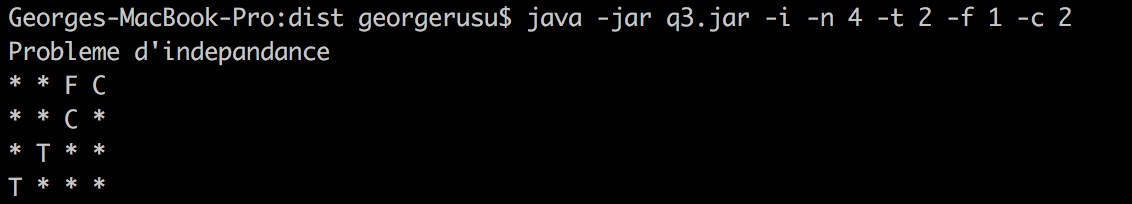
\includegraphics[width=\linewidth]{img/q3.png}
  \caption{Exemple de lancement problème independance}
\end{figure}
\par où
\begin{enumerate}
	\item[-] -i si c'est le problème d'indépendance
	\item[-] -d si c'est le problème de domination
	\item[-] -n 4 pour la taille de l'échiquier (ici nous avons défini une taille de 4)
	\item[-] -t 2 pour le nombre de pièce Tour (ici 2)
	\item[-] -f 1 pour le nombre de pièce Fou (ici 1)
	\item[-] -c 2 pour le nombre de Cavalier (ici 2)
\end{enumerate}

Encore un exemple d'utilisation, cette fois-ci pour le problème de domination:
\begin{figure}[!h]
  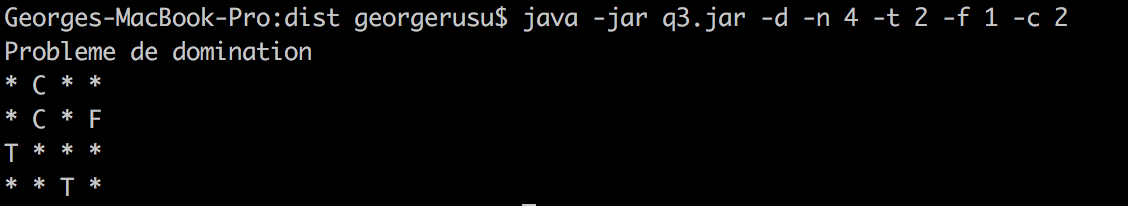
\includegraphics[width=\linewidth]{img/q31.png}
  \caption{Exemple de lancement problème domination}
\end{figure}
\subsection{Explication code}
\par Pour cette question nous avons créé un package "allPiece" qui va contenir les classes lié a une pièce et un package "question3Choco" qui est le package où se trouve la classe "Main" principale ainsi que la classe "Jeu" qui lance le tout. 

\par Le fonctionnement se passe ainsi, pour n'importe quel type de problème, on va instancier le nombre exact de pièce de type Tour, Cavalier, Fou et Vide. Nous allons mettre chacun de ces objets dans un tableau et on va parcourir ce tableau de telle manière à jouer avec chaque pièce. Nous vérifions bien le fait qu'on ne traite pas la même pièce avec elle même (auto menacement). Nous avons aussi une contraintes concernant la position de chaque pièces, deux pièces ne peuvent pas avoir la meme position puisqu'elle doivent etre distincte.
\par Si le problème est une celui de l'indépendance, une pièce ne peut pas s'auto menacer et ne peut pas menacer les autres pièces non Vide. Voici le pseudo code:
\begin{lstlisting}[language=Java,basicstyle=\tiny]
if (l!=k){ //si pas la meme piece
	Piece pieceAttaque=allPiece.get(l); //premiere piece
	Piece pieceSubit=allPiece.get(k); //deuxieme piece
					
	Constraint unique=pieceAttaque.unique(pieceSubit); //contrainte d'unicite
	unique.post();
					
	if ((pieceAttaque.getType()!="*") && (pieceSubit.getType()!="*")){
		//si il ne s'agit pas d'une piece qui vide qui attaque une piece vide
		Constraint attaque= model.not(pieceAttaque.Menace(pieceSubit));
		attaque.post();	
	}
}
\end{lstlisting}

\par Maintenant regardons pour le problème de domination. En plus du fait que c'est la negation de la domination ($\neg \neg x=x$) il faut gérer le cas lorsqu'il y a des obstacles pour les Tours et Fous. Si il y a quelques choses entre la cible et une Tour alors celle-ci ne sera pas menacé. Il s'agit pour ce cas d'un problème d'indépendance pour les Tours et les Fous. Voici le pseudo code:
\begin{lstlisting}[language=Java,basicstyle=\tiny]
if (l!=k){ //si pas meme piece
	Piece pieceAttaque=allPiece.get(l); //premiere piece
	Piece pieceSubit=allPiece.get(k); //seconde piece
		
	Constraint unique=pieceAttaque.unique(pieceSubit);
	unique.post(); //position unique
			
	if ((pieceAttaque.getType()=="*") && (pieceSubit.getType()!="*")){
		//si un case vide alors elle doit etre menace
		Constraint attaque = pieceSubit.Menace(pieceAttaque); 
		//case non vide menace une case vide
		OR_contraintes.add(attaque);
	}
	if ((pieceAttaque.getType()=="T") && (pieceSubit.getType()=="F")){
		//gestion des obstacles pour Tour et pour Fou
		Constraint attaque = model.not(pieceAttaque.Menace(pieceSubit));
		OR_contraintes.add(attaque);
	}
}
\end{lstlisting}

\par Au niveau des contraintes, on fait un OR de toutes les contraintes dans les deux cas de figures.

\subsection{Contrainte Tour}
\par Regardons à present la classe Tour du package allPiece. Les contraintes pour dire qu'une Tour menace une pièce sont tres simple. Regadons d'abord le pseudo code:

\begin{lstlisting}[language=Java,basicstyle=\tiny]
public Constraint Menace(Piece pieceCible){
	Model model=this.getModel();
	Constraint memeLigne=model.arithm(this.getCoordLigne(), "=", pieceCible.getCoordLigne());
	Constraint memeColonne=model.arithm(this.getCoordColonne(), "=", pieceCible.getCoordColonne());
	return model.or(memeLigne,memeColonne);
}
\end{lstlisting}
 En d'autres termes, nous disons tout simplement qu'une pièce ne peut pas avoir la meme ligne ou la meme colonne qu'une pièce tour si elle veut ne pas etre menacé par celle-ci.
\subsection{Contrainte Fou}
\par Regardons la classe Fou du package allPiece pour comprendre comment fonctionne les contraintes pour le type de pièce Fou.
\begin{lstlisting}[language=Java,basicstyle=\tiny]
public Constraint Menace(Piece pieceCible){
 Model model=this.getModel();
 Constraint constraint =model.arithm(this.getCoordColonne().sub(pieceCible.getCoordColonne()).abs().intVar(),
 "=",this.getCoordLigne().sub(pieceCible.getCoordLigne()).abs().intVar());
	   
 return constraint;
}
\end{lstlisting}

Pour cette contrainte nous nous basons sur ce que le professeur a donné en cours concernant le jeu des 8 reines. Verifier qu'une pièce a la meme diagonale qu'une autre revient a faire $|i-k|=|j-l|$ avec $(i,j)$ les coordonne de la premier pièce et $(k,l)$ les coordonne de la seconde pièce.

\subsection{Contrainte Cavalier}
Pour ce dernier type de pièce, procedons de la meme maniere. Le pseudo code:
\begin{lstlisting}[language=Java,basicstyle=\tiny]
public Constraint Menace(Piece pieceCible){
	Model model=this.getModel();
	ArrayList<Constraint> cavalierAttaque=new ArrayList<Constraint>();
		
	//i+1 j+2
	Constraint memeLigne=model.arithm(this.getCoordLigne().add(1).intVar(), "=", pieceCible.getCoordLigne());
	Constraint memeColonne=model.arithm(this.getCoordColonne().add(2).intVar(), "=", pieceCible.getCoordColonne());
	cavalierAttaque.add(model.and(memeLigne,memeColonne));
	
	//i+1 j-2
	memeLigne=model.arithm(this.getCoordLigne().add(1).intVar(), "=", pieceCible.getCoordLigne());
	memeColonne=model.arithm(this.getCoordColonne().sub(2).intVar(), "=", pieceCible.getCoordColonne());
	cavalierAttaque.add(model.and(memeLigne,memeColonne));
		
	//i-1 j+2
	memeLigne=model.arithm(this.getCoordLigne().sub(1).intVar(), "=", pieceCible.getCoordLigne());
	memeColonne=model.arithm(this.getCoordColonne().add(2).intVar(), "=", pieceCible.getCoordColonne());
	cavalierAttaque.add(model.and(memeLigne,memeColonne));
	
	//i-1 i-2
	memeLigne=model.arithm(this.getCoordLigne().sub(1).intVar(), "=", pieceCible.getCoordLigne());
	memeColonne=model.arithm(this.getCoordColonne().sub(2).intVar(), "=", pieceCible.getCoordColonne());
	cavalierAttaque.add(model.and(memeLigne,memeColonne));
	
	//i+2 j+1
	memeLigne=model.arithm(this.getCoordLigne().add(2).intVar(), "=", pieceCible.getCoordLigne());
	memeColonne=model.arithm(this.getCoordColonne().add(1).intVar(), "=", pieceCible.getCoordColonne());
	cavalierAttaque.add(model.and(memeLigne,memeColonne));
	
	//i+2 j-1
	memeLigne=model.arithm(this.getCoordLigne().add(2).intVar(), "=", pieceCible.getCoordLigne());
	memeColonne=model.arithm(this.getCoordColonne().sub(1).intVar(), "=", pieceCible.getCoordColonne());
	cavalierAttaque.add(model.and(memeLigne,memeColonne));
	
	//i-2 j+1
	memeLigne=model.arithm(this.getCoordLigne().sub(2).intVar(), "=", pieceCible.getCoordLigne());
	memeColonne=model.arithm(this.getCoordColonne().add(1).intVar(), "=", pieceCible.getCoordColonne());
	cavalierAttaque.add(model.and(memeLigne,memeColonne));
	
	//i-2 j-1
	memeLigne=model.arithm(this.getCoordLigne().sub(2).intVar(), "=", pieceCible.getCoordLigne());
	memeColonne=model.arithm(this.getCoordColonne().sub(1).intVar(), "=", pieceCible.getCoordColonne());
	cavalierAttaque.add(model.and(memeLigne,memeColonne));
	
	return model.or(cavalierAttaque.toArray(new Constraint[]{}));
}
\end{lstlisting}

Ce qu'on fait ici c'est tout simplement dire que pour un cavalier, la pièce qui est menacé par ce cavalier doit se trouver à la position du saute du cavalier.

\subsection{Contrainte Vide}
Nous nous sommes rendu compte qu'on a besoin de cette classe juste pour certaintes fonctionne comme l'affichage et comme la verification qu'une pièce qui doit attaque ou qui se fait attaquer n'est pas une pièce vide. Il n'y a donc aucun intérêt a montrer les contraintes dans ce cas puisqu'il ne renvoi qu'un null, on n'utilise jamais cette fonction menace pour ce type de pièce mais puisque nous avons choisi de faire une classe abstraite pour toutes les pièces, il a été nécessaire de devoir redéfinir cette méthode ici.

Ce qui ne faut pas oublier de mentionner c'est que cette classe nous sert également pour les positions. En effet le fait de verifier a chaque fois que chaque pièce est distincte oblige l'utilisation des pièces Vides qui ont, elles aussi une position.

\subsection{Question Bonus}
\par Pour cette question bonus, il nous a été demander de pouvoir laisser le choix a un utilisateur de définir lui meme un type de pièce. Pour cela nous avons simuler un utilisateur qui creer une classe Pion. Cette classe tout comme les autres pièces herite de la classe abstraite Piece et doit definir imperativement la methode: \textit{public Constraint Menace(Piece pieceCible)\{\}}

Voici ce que nous avons defini pour le type de pièce Pion:

\begin{lstlisting}[language=Java,basicstyle=\tiny]
public Constraint Menace(Piece pieceCible){
	Model model=this.getModel();
	ArrayList<Constraint> pionAttaque=new ArrayList<Constraint>();
	
	//i+1 j+1
	Constraint memeLigne=model.arithm(this.getCoordLigne().add(1).intVar(), "=", pieceCible.getCoordLigne());
	Constraint memeColonne=model.arithm(this.getCoordColonne().add(1).intVar(), "=", pieceCible.getCoordColonne());
	pionAttaque.add(model.and(memeLigne,memeColonne));
	//i+1 j-1
	memeLigne=model.arithm(this.getCoordLigne().add(1).intVar(), "=", pieceCible.getCoordLigne());
	memeColonne=model.arithm(this.getCoordColonne().sub(1).intVar(), "=", pieceCible.getCoordColonne());
	pionAttaque.add(model.and(memeLigne,memeColonne));
	
	//i-1 j+1
	memeLigne=model.arithm(this.getCoordLigne().sub(1).intVar(), "=", pieceCible.getCoordLigne());
	memeColonne=model.arithm(this.getCoordColonne().add(1).intVar(), "=", pieceCible.getCoordColonne());
	pionAttaque.add(model.and(memeLigne,memeColonne));
	
	//i-1 i-1
	memeLigne=model.arithm(this.getCoordLigne().sub(1).intVar(), "=", pieceCible.getCoordLigne());
	memeColonne=model.arithm(this.getCoordColonne().sub(1).intVar(), "=", pieceCible.getCoordColonne());
	pionAttaque.add(model.and(memeLigne,memeColonne));
	
	return model.or(pionAttaque.toArray(new Constraint[]{}));
}
\end{lstlisting}

Au echec le pion peut aller dans une seule direction, nous avons voulu dresser le cas ou c'est un pion qui par dans toutes les directions. Pour pouvoir faire fonctionner ce Pion, l'utilisateur devra modifier le fichier Main.java afin d'ajouter la possibilité de specifier le nombre de Pion et d'utiliser ce nombre dans la classe Jeu.java afin de creer le nombre d'instance necessaire et de les ajouter dans le tableau avec toutes les pièces. Par la suite il pourra tester son programme avec le nouveau type de pièce ajouté.
\section{Question 4}
\par Pour cette question nous avons dut implementer une programme qui pour une grille de taille n va nous donner le nombre minimal de cavalier afin que le problème de domination\footnote{soit une case est occupé soit elle est menacé} soit respecté. Nous sommes parti sur une matrice de IntVar de taille $n*n$ avec pour chaque case un domaine compris entre 0 et 1. Nous avons defini au prealable qu'une case ayant un 0 sera consideré comme vide et inversement une case contenant un 1 sera consideré comme remplie par un et un seul cavalier. 
\subsection{Contraintes}
\par Afin de pouvoir minimiser, nous devons ajouter nos contraintes. Nous pouvons nous aider du fait qu'une case ne peut que soit être vide, soit contenir un cavalier. Nous allons donc pour chaque case parcourir la matrice de IntVar\footnote{cette matrice represente la grille que nous devons dominer avec le moins de cavalier possible} et ajouter les contraintes de la facon suivante:
\begin{lstlisting}[language=Java,basicstyle=\tiny]
public Constraint menace(int ligne,int colonne){
	ArrayList<Constraint> cavalierAttaque=new ArrayList<Constraint>();
		
	//i+1 j+2
	if ((ligne+1<this.n) && (colonne+2<this.n)){
		Constraint menace=this.model.arithm(this.echequier[ligne+1][colonne+2], "!=", this.echequier[ligne][colonne]);
		cavalierAttaque.add(menace);
	}
	//i+1 j-2
	if ((ligne+1<this.n) && (colonne-2>=0)){
		Constraint menace=this.model.arithm(this.echequier[ligne+1][colonne-2], "!=", this.echequier[ligne][colonne]);
		cavalierAttaque.add(menace);
	}
	
	//i-1 j+2
	if ((ligne-1>=0) && (colonne+2<this.n)){
		Constraint menace=this.model.arithm(this.echequier[ligne-1][colonne+2], "!=", this.echequier[ligne][colonne]);
		cavalierAttaque.add(menace);
	}
	
	//i-1 j-2
	if ((ligne-1>=0) && (colonne-2>=0)){
		Constraint menace=this.model.arithm(this.echequier[ligne-1][colonne-2], "!=", this.echequier[ligne][colonne]);
		cavalierAttaque.add(menace);
	}
	//i+2 j+1	
	if ((ligne+2<this.n) && (colonne+1<this.n)){
		Constraint menace=this.model.arithm(this.echequier[ligne+2][colonne+1], "!=", this.echequier[ligne][colonne]);
		cavalierAttaque.add(menace);
	}
	//i+2 j-1
	if ((ligne+2<this.n) && (colonne-1>=0)){
		Constraint menace=this.model.arithm(this.echequier[ligne+2][colonne-1], "!=",this.echequier[ligne][colonne]);
		cavalierAttaque.add(menace);
	}
	//i-2 j+1
	if ((ligne-2>=0) && (colonne+1<this.n)){
		Constraint menace=this.model.arithm(this.echequier[ligne-2][colonne+1], "!=",this.echequier[ligne][colonne]);
		cavalierAttaque.add(menace);
	}
	//i-2 j-1
	if ((ligne-2>=0) && (colonne-1>=0)){
		Constraint menace=this.model.arithm(this.echequier[ligne-2][colonne-1], "!=", this.echequier[ligne][colonne]);
		cavalierAttaque.add(menace);
	}
	if (!cavalierAttaque.isEmpty()){
		return this.model.or(cavalierAttaque.toArray(new Constraint[]{}));
	}
	return null;
		
	}
\end{lstlisting}

Ce que nous fesons ici c'est tout simplement dire que pour chaque case, la case attaquante respective, donc la case où doit se trouver un cavalier doit etre differente d'elle meme. En effet nous avons que deux valeurs dans le domaines de chaque cases ce qui nous laisse l'opportunité de jouer avec la difference entre la case cible et cèlle qui attaque.

Voici comment nous ajoutons nos contraintes et comment nous definison la variable a minimiser:
\begin{lstlisting}[language=Java,basicstyle=\tiny]
public void MinimizationCavalier(){
	for (int l=0;l<this.n;l++){
		for (int k=0;k<this.n;k++){
			if (this.menace(l,k)!=null){ //si il existe une contrainte
				this.menace(l,k).post();
			}
			else{
				this.model.arithm(this.echequier[l][k], "=",1).post(); //sinon c'est une case occupe ->cavalier
			}
			this.sum=this.sum.add(this.echequier[l][k]).intVar();
		}	
	}
	this.numCavalier.eq(sum).post();
	this.model.setObjective(Model.MINIMIZE, this.numCavalier);
	[...]
}
\end{lstlisting}

Puisque a nouveau si une case contient un cavalier, sa valeur sera egale a 1 ou 0 dans le cas d'une case vide, nous ajoutons la contrainte que la somme de toutes les cases doit etre egale au nombre de cavalier qu'on doit minimiser.

\subsection{Exemple d'utilisation}
Voici un exemple d'utilisation:
\begin{figure}[!h]
  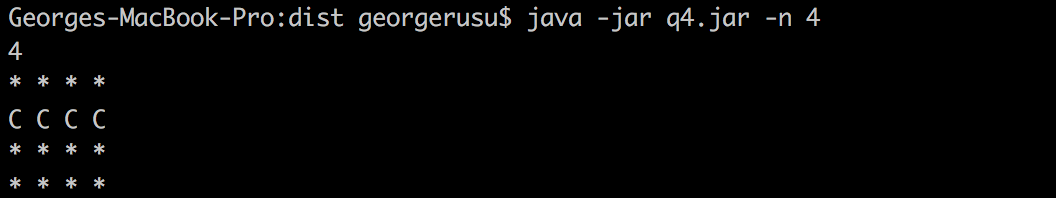
\includegraphics[width=\linewidth]{img/q4.png}
  \caption{Exemple de lancement problème independance}
\end{figure}

\section{Question 5}
\subsection{Contraintes CSP}
	Nous avons un musée qui est reprséenté par une grille de $n * m$\\
	\textbf {Variables de décision} $ X = \{x_{i,j} | \forall i,j (1 \leq i \leq n).(1 \leq j \leq m)\}$\\
	\textbf{Domaines : } $ D = \{0, 1, 2, 3, 4, 5\} $ correspondant respectivement à une case vide, une caméra Nord, une caméra Sud, une caméra Est, une caméra Ouest et un mur.\\
	\textbf{Contraintes : } La contrainte du musée est définie comme ceci: chaque case vide doit être surveillé par au moins une caméra. La solution doit être trouvée avec un nombre de caméra le plus petit possible.

		Pour appliquer la contrainte, il faut donc prendre en compte chaque case du musée.  Pour cela nous prenons chaque $x_{i,j}$ compris dans la taille du musée. Ensuite il faut vérifier que pour chacune de ces cases, si elle est non occupée, il faut qu'elle soit surveillé par au moins une caméra.  Ainsi nous avons une suite d'ensemble de valeurs liées par des relations \emph{OR}, qui nous permet de dire: existe au moins une caméra observant la case vide.

		Afin d'être sûr qu'une caméra pointe vers le bon sens, lorsque nous parcourons les lignes et colognes d'une case vide, nous précisons bien qu'il y ai au moins une caméra regardant vers le Nord dans les cases se trouvant en dessous de notre case $x_{i,j}$, et ainsi de suite pours les autres directions.
		$$ C = ((x_{i,j}, \forall i,j(1 \leq i \leq n ).(1 \leq j \leq m)),\{b_{i,j},\forall i,j(1 \leq i \leq n ).(1 \leq j \leq m)| [(b_{i,j} = 0) \land (\forall k (i < k \leq n), \exists b_{k,j} = 1)] \lor $$
		$$ [(b_{i,j} = 0) \land (\forall k (0 \leq k < i), \exists b_{k,j} = 2)] \lor $$
		$$ [(b_{i,j} = 0) \land (\forall k (j < k \leq m), \exists b_{i,k} = 3)] \lor $$
		$$ [(b_{i,j} = 0) \land (\forall k (0 \leq k < j), \exists b_{i,k} = 4)] \}) $$

		Afin de réduire le nombre de caméra, nous avons reformulé de la demande d'optimisation.  C'est à dire que nous n'allons plus chercher à minimiser le nombre de caméra, mais à maximiser le nombre de case surveillé, ce qui équivaut à la même solution. En effet en réduisant le nombre de caméra, on maximise le nombre de case surveillé avec un petit nombre de caméra.

		Il n'y a donc pas de contrainte \emph{CSP} à écrire.  Il suffit de donner dire au programme de trouver la solution avec le plus de case vide possible.

	\subsection{Partie implémentation}
		\subsubsection{Parser}
			La première chose à faire pour résoudre le problème de minimisation du nombre de caméra dans un musée, et de donner au programme l'architecture du musée.  C'est à dire donner au programme une carte représentant les murs et les trous à surveiller / combler par des caméras.

			Pour ce faire le programme prend en paramètre d'éxécution un fichier texte sous le format suivant:
			\begin{figure}[h]
			\begin{center}
				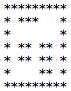
\includegraphics{img/gridExample.png}
			\end{center}
			\end{figure}

			Une fois que le programme récupère ce fichier, il va récupérer tout d'abord les dimensions du musée sans compter les quatres mur de la pièce.  Une fois terminé, ces valeurs sont donnée aux attributs du programme. Une matrice \emph{grid} est ensuite crée.  Cette matrice représente la situation de la pièce du musée avec les murs, et permettra ainsi au programme de placer les caméras aux bons endroits.

		\subsubsection{Placements des caméras}
			Maintenant que la matrice \emph{grid} à été initialiser, nous pouvons appliquer nos contraintes en fonction de chaque case de cette matrice. Nous faisons alors appel à \emph{minCamera()}, qui va parcourirs chaque case de notre matrice.  Si la case est différent de "*", qui correspond à un mur, alors nous allons appliquer des contraintes. Pour ce faire nous initialisons un tableau qui va contenir toutes nos contraintes, ce tableau est \emph{contrainteTotal\_OR}. C'est ce tableau qui va permettre d'indiquer au solver, si une case est vide, alors elle est surveillé par au moins une caméra. Ensuite pour la case vide, il va falloir dire: il existe au moins une caméra Sud dans les cases au dessus de notre case vide, ou alors une caméra Nord dans les cases en dessous, ou alors une caméra Est dans les cases à gauche, ou une caméra Ouest dans les cases à droite.  Pour ce faire on crée à nouveau un tableau (\emph{existsCam\_OR}) qui va contenir ces contraintes. On parcours alors en croix les cases adjacentes à la case vide, en prenant soin de nous arrêter lorsque nous rencontrons un mur. Lors de ce parcours, nous ajoutons à notre tableau la contrainte arithmétique: case parcouru $=$ caméra visant notre case vide. Une fois le parcours en croix terminé, il suffit d'ajouter au tableau \emph{contrainteTotal\_OR} quatre contraintes indiquant que la case que nous examinons peut aussi être remplit par une caméra. Il ne reste plus qu'à poster les contraintes du tableau grâce à un \emph{post()} de notre tableau.

		\subsubsection{Affichage de la solution}
			Pour afficher la solution, il ne reste plus qu'à parcourirs le tableau contenant les différentes positions des caméras utilisé par le solver (\emph{this.salle}).  Ce tableau contient la structure de la salle, les cases vides, et le entiers correspondant au caméra et leur sens.

		\subsubsection{Exemple}
			\begin{figure}[h]
			\begin{center}
				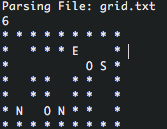
\includegraphics[scale=0.7]{img/sol.png}
			\end{center}
			\end{figure}
\end{document}